\documentclass{article}
\usepackage{graphicx}
\usepackage[left=1in, right=1in, top=1in, bottom=1in]{geometry}
\usepackage[utf8]{inputenc}
\usepackage[spanish]{babel}
\selectlanguage{spanish}
\spanishdecimal{.}
\usepackage{titling}
\usepackage{lipsum}
\title{Actividad 4: Introducción a matplotlib}
\author{Borbón Fragoso Julio César }
\date{16 Febrero del 2019}

\begin{document}

\maketitle

\section{Introducción}

Matplotlib es una libreria de Python que produce cierta variedad de figuras acerca de un arreglo de datos de maneras distintas. Su propósito es hacer más facil el realizar un análisis de datos mediante figuras con unas pocas lineas de codigo con ella puedes generar gráficas, histogramas, gráficas de barras, diagramas de caja, etc. En nuestro caso continuando la actividad realizada anteriormente realizaremos algunas figuras del comportamiento del clima de la ciudad de Sahuria, Sonora. 

\section{Realizando la actividad}
La actividad consistio en 5 partes que se intentaran detallar de la manera más breve y completo posible a continuación.
\subsection{Gráfica de barras de la precipitación acumulada promedio mensual}
Con la ayuda de un dataframe realizado con pandas en la actividad anterior que nos permitia acomodar los datos de cierta manera por años o por mes de una columna de datos queria se realizo esta gráfica con la siguiente linea:
 \begin{verbatim} 
 axx = df11.plot.bar(x='PRECIP', y='FECHA', rot=0)
 \end{verbatim}
 Y la gráfica de barras que nos dio se da a continuación:  \\
 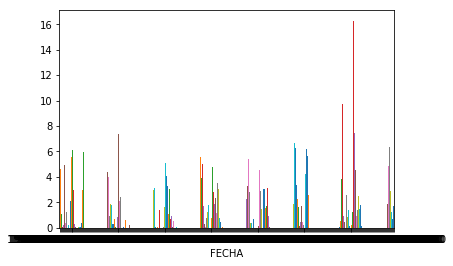
\includegraphics[scale=.85]{barrasprecipmensual.png}
 
 \subsection{Gráfica de barras de la precipitación acumulada promedio anual}
 De la misma manera que la anterior, con ayuda de un dataframe con pandas, se utilizo el siguiente codigo para generar una barplot.
  \begin{verbatim} 
  ax = df10.plot.bar(x='PRECIP', y='FECHA', rot=0)
   \end{verbatim}
Y la gráfica resultante se da a continuación:  \\
 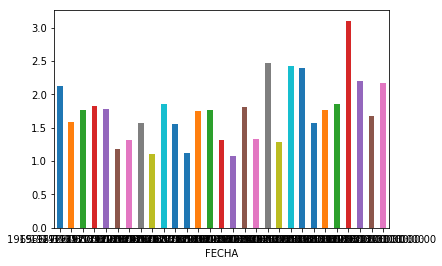
\includegraphics[scale=.85]{barrasprecipanual.png}

\subsection{Gráfica de evolución de la temperatura máxima y minima}
Con el primer dataframe de datos realizado en la actividad anterior se realizo la gráfica solicitada con el siguiente codigo:
\begin{verbatim}
    df9.plot(x="FECHA",y=["TMAX","TMIN"])
\end{verbatim}
Con la siguiente gráfica resultante: \\
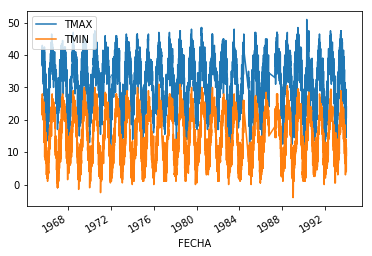
\includegraphics[scale=.85]{evoluciondetmaxtmin.png}

\subsection{Gráfica de cajas de TMAX y TMIN, mensuales separadas}
Se genero un nuevo dataframe con las características solicitadas, se volvieron númericas las columnas "TMAX", "TMIN" y se útilizo la siguiente linea de codígo:
\begin{verbatim}
df12.boxplot(column=['TMAX'])
df12.boxplot(column=['TMIN'])
\end{verbatim}
Y se generaron los siguientes 2 diagramas de cajas: \\

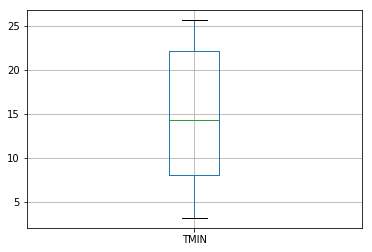
\includegraphics[scale=.7]{cajatminmensual.png}
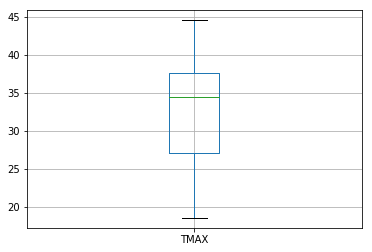
\includegraphics[scale=.7]{cajatmaxmensual.png}

\subsection{Gráficas de cajas de TMAX y TMIN, anuales separadas}
De la misma manera que antes, se genero un nuevo dataframe y las columnas necesarias se tornaron númericas y se utilizo la siguiente linea de codígo:
\begin{verbatim}
    df13.boxplot(column=['TMAX'])
    df13.boxplot(column=['TMIN'])
\end{verbatim}
Y se nos dieron los 2 siguientes diagramas: \\
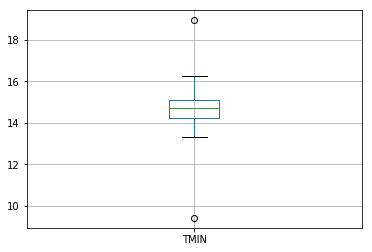
\includegraphics[scale=.7]{cajatminanual.png}
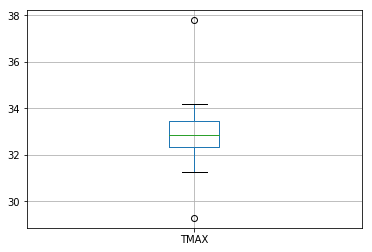
\includegraphics[scale=.7]{cajatmaxanual.png}

\section{Conclusión}
Se concluye que con el uso de Matplotlib y la ayuda de pandas se puede realizar de una manera más sencilla la visualización de datos mediante diversas figuras que nos dan una idea del comportamiento de estos mismos.


\end{document}
